% Created 2021-05-12 Wed 21:47
% Intended LaTeX compiler: pdflatex
\documentclass[9pt, b5paper]{article}
\usepackage[UTF8]{ctex}
\usepackage{fontspec}
\usepackage{graphicx}
\usepackage{xcolor}
\usepackage{multirow}
\usepackage{multicol}
\usepackage{float}
\usepackage{textcomp}
\usepackage{geometry}
\geometry{left=1.2cm,right=1.2cm,top=1.5cm,bottom=1.2cm}
\usepackage{algorithm}
\usepackage{algorithmic}
\usepackage{latexsym}
\usepackage{natbib}
\usepackage{listings}
\usepackage{minted}
\usepackage[xetex,colorlinks=true,CJKbookmarks=true,linkcolor=blue,urlcolor=blue,menucolor=blue]{hyperref}
\author{deepwaterooo}
\date{\today}
\title{成长的故事 —— 我和表哥}
\hypersetup{
 pdfauthor={deepwaterooo},
 pdftitle={成长的故事 —— 我和表哥},
 pdfkeywords={},
 pdfsubject={},
 pdfcreator={Emacs 27.1 (Org mode 9.3)}, 
 pdflang={English}}
\begin{document}

\maketitle
\tableofcontents


\section{2013 Summer Intern暑假实习(6)—— 交叉项目:人际交叉、公司栽脏爆点、炒作职场非正常男女关系舆论}
\label{sec:org1513e14}

前面写到了:实习生暑假实习期间正常更换实习导师、被三星公司高层组长C等刻意安排、制造舆论、炒作成了:实习生我处理不好与三星公司正式员工、mentor senior长老B的职场人际关系,迫使公司不得不为我这个事端制造者更换了导师。 

\begin{center}

\includegraphics[width=.9\linewidth]{./pic/backups_plans_20210511_101118.png}
\end{center}

上个周是属于实习生实习期间换mentor、公司自导自演又上演了一出三在中文炒作舆论的燃点爆点。

\begin{center}

\includegraphics[width=.9\linewidth]{./pic/backups_plans_20210511_102103.png}
\end{center}

公司里的领导自己的样子倒是做得很好的,该道歉的道歉,但是被他们故意炒作、作贱、被剥夺了生存资源的职场年轻女性的生存空间呢?是他们为官的假惺惺一句道歉就可以解决得了的吗?

\begin{center}

\includegraphics[width=.9\linewidth]{./pic/backups_plans_20210511_102539.png}
\end{center}

更何况,就像表姐所陈述清楚的,她只是善常体察上意,将上层领导们需要、想要她帮招进来的那些个公司里的易燃易爆品招募了进来。

\begin{center}

\includegraphics[width=.9\linewidth]{./pic/backups_plans_20210511_102727.png}
\end{center}

而他们、公司上层自然是清楚地、仔细地打听过他们所招员工(比如那个暑假专门用来拖住我、对付我的、缺乏专业素养的长老B)的人品、素质、工作表现等方方面面!!

你以为他们这次的换导师事件只是各种情形之下的一件事发突然吗?

不,他们有专业的故意制造燃点爆点舆论踢爆炒作小分队、他们接下来仍然会(利用他们为我组装的小伙伴队伍的口舌、警犬尖人、表姐等)一再造谣、一再人为刻意制造燃点、爆点,并利用合用三大中文媒体喉舌的力量将这股舆论彻底炒爆、炒出他们三星公司所想要达到的他们曾经多么地仁义、公道、曾经多么仁慈地站出来救助过的人道主义立场!!!

接下来,我们还是先看项目上的进展。 

\begin{center}

\includegraphics[width=.9\linewidth]{./pic/backups_plans_20210511_105354.png}
\end{center}

这里应该是存在一些笔误:就是这是前导师长老B一个周前给布置的交叉项目,现在是暑假后半段新换导师、前文称呼正式员工A帮忙review. 

\begin{center}

\includegraphics[width=.9\linewidth]{./pic/backups_plans_20210511_105634.png}
\end{center}

\begin{center}

\includegraphics[width=.9\linewidth]{./pic/backups_plans_20210511_105715.png}
\end{center}

这里的笔误是,这个项目不是要从一个文件,而是从多个文件。回忆起来某些不太显眼不太重要的事件的先后顺序可能会有错乱,在所难免。这个小细节就此指出,不必过于在意。 

那么这个上个周所布置的交叉项目、前导师长老B所留下的上个周的项目,新导师A会如何帮我review呢?

\begin{center}

\includegraphics[width=.9\linewidth]{./pic/backups_plans_20210511_110111.png}
\end{center}

换导师后新一周的周一还是周二的中午偏下午一两点钟(?),新导师A就帮稍微点评了一下代码乱在哪里,可以先从哪些方面作些改进。

\begin{center}

\includegraphics[width=.9\linewidth]{./pic/backups_plans_20210511_110130.png}
\end{center}

\begin{center}

\includegraphics[width=.9\linewidth]{./pic/backups_plans_20210511_110510.png}
\end{center}

\begin{center}

\includegraphics[width=.9\linewidth]{./pic/backups_plans_20210511_110559.png}
\end{center}

从小喜欢学《数学》、《化学》等非语言文字学科、学过《统计》硕士专业,经历过统计专业29个月的OPT实习,我应该总是对自己分析解决问题的能力还是比较肯定、有着很大程度上的自信的吧。 

\begin{center}

\includegraphics[width=.9\linewidth]{./pic/backups_plans_20210511_110329.png}
\end{center}

这里,我又一次自信地(或者说是自大地)估计了一个一个小时之内解决掉导师A所提出的建议问题的(改混乱代码成为一个module),却意识不到这是一个考验的开始。 

\begin{center}

\includegraphics[width=.9\linewidth]{./pic/backups_plans_20210511_111340.png}
\end{center}

但那时,我真的认为我不是在骄傲,而是心里面有一种急——如果这个导师的编程能力真的很强大,那么作为我亲爱的表哥眼中少女心小弱弱的我,是很想要抓住这个机会多从这样一个职场专业人士的guidence里多学习点儿新知识、新经验或者是能够被他培养出多一些计算机专业里的能力的。

我很急,我想要尽快、估莫着一个小时左右把事情做完,好可以把这个项目干完了结、好可以从导师A那里请他帮忙想出、我可以索要得到新任务、或者更多的任务与专业锻炼。 

\begin{center}

\includegraphics[width=.9\linewidth]{./pic/backups_plans_20210511_111704.png}
\end{center}

但是很显然,作为python语言的小儿科弱弱,我还是严重低估了它的难度,修改的过程中也出现过各种各样的问题,一两个小时后到那天下午三四点钟的时候,我已经有些沉不住气,跑去同新导师A交换一下意见了。 

\begin{center}

\includegraphics[width=.9\linewidth]{./pic/backups_plans_20210511_111728.png}
\end{center}

我这样跑去问导师A,是有点儿打扰他了。但当时的自己已经感到压力了,需要与导师交换一下观点意见、作些调整吧。

\begin{center}

\includegraphics[width=.9\linewidth]{./pic/backups_plans_20210511_112426.png}
\end{center}

新导师A说等他忙完再去帮我看看。而我、稍微减压后还是得回去继续修改自己的代码。 

\begin{center}

\includegraphics[width=.9\linewidth]{./pic/backups_plans_20210511_112554.png}
\end{center}

又过了约两个小时左右,当傍晚六点钟,导师A不得不下班的时候,他过来察看我的进展。 

\begin{center}

\includegraphics[width=.9\linewidth]{./pic/backups_plans_20210511_112718.png}
\end{center}

恩,又过了两个小时,又整了两个小时之后,我终于是把那个python module的入门级知识点、考点儿给过了!

\begin{center}

\includegraphics[width=.9\linewidth]{./pic/backups_plans_20210511_110559.png}
\end{center}

新导师A还比较开心,他那天已经到下班时间要回家了,他答应第二天就帮我review. 新导师A会帮我想出来、会安排我做的下一个项目会是什么呢?到那时,我应该还是很开心很向往的吧,一如当年几个月前的春天AI人工智能课结束、清楚地感受了一个学期这门课代课老师的分析能力与授课知识点的透彻性,我已经向代课老师上课提问示好(明示问题示好),表达了我跟他做科研的兴趣,期望以后能有机会跟他一起作课题!

\begin{center}

\includegraphics[width=.9\linewidth]{./pic/backups_plans_20210511_114253.png}
\end{center}

那个周二的下午,三四个小时,只为解决、fix掉一个learning curve偏低的python的一个基础级的module入门考点bug。那三四个小时,自已的亲身体会、真切感受如何?

\begin{center}

\includegraphics[width=.9\linewidth]{./pic/backups_plans_20210511_114322.png}
\end{center}

这里,当新导师A给我更多的时间让我学着去自己解决问题,我能够感受到自己需要努力,也能够做到在心里鼓励自己更加努力。 

\begin{center}

\includegraphics[width=.9\linewidth]{./pic/backups_plans_20210511_114411.png}
\end{center}

这里确实是一个基础,如果导师A同任何其它庸俗碌碌辈一样、同先前长老B凡事不会就去问其它组其它同事一样,那我们实习生实习期间的专业能力、是很难得到成长与提升的。 

这个基础——互相站在对方的立场上试图去为对方想一想、并相信对方的做法一定是为自己好的、是有他自己一定道理的,确实是垫定了实习期间这个导师与实习生我之间相互理解信任的mentor-guidence合作基础。

我们来回忆一下我亲爱的表哥与我建立信任基础、爱情基础、到树立起坚定的爱情信念的那些个感动瞬间。 

\begin{center}

\includegraphics[width=.9\linewidth]{./pic/backups_plans_20210511_115910.png}
\end{center}

2010年2月,当《统计》专业的我硕士毕业,就要前去加州找工作了,走之前路过表哥家,把一两样不太重要的东西留下,却发现我亲爱的表哥从他的车里钻出来,送我出门呢!

\begin{center}

\includegraphics[width=.9\linewidth]{./pic/backups_plans_20210511_120022.png}
\end{center}

但是到了加州之后,我对我亲爱的表哥爱情的点点星火就被大表姐给亲手掐灭了。 

\begin{center}

\includegraphics[width=.9\linewidth]{./pic/backups_plans_20210511_120208.png}
\end{center}

\begin{center}

\includegraphics[width=.9\linewidth]{./pic/backups_plans_20210511_120306.png}
\end{center}

\begin{center}

\includegraphics[width=.9\linewidth]{./pic/backups_plans_20210511_120425.png}
\end{center}

\begin{center}

\includegraphics[width=.9\linewidth]{./pic/backups_plans_20210511_120500.png}
\end{center}

\begin{center}

\includegraphics[width=.9\linewidth]{./pic/backups_plans_20210511_120655.png}
\end{center}

\begin{center}

\includegraphics[width=.9\linewidth]{./pic/backups_plans_20210511_120730.png}
\end{center}

\begin{center}

\includegraphics[width=.9\linewidth]{./pic/backups_plans_20210511_120816.png}
\end{center}

\begin{center}

\includegraphics[width=.9\linewidth]{./pic/backups_plans_20210511_120902.png}
\end{center}

\begin{center}

\includegraphics[width=.9\linewidth]{./pic/backups_plans_20210511_120952.png}
\end{center}

\begin{center}

\includegraphics[width=.9\linewidth]{./pic/backups_plans_20210511_121705.png}
\end{center}

\begin{center}

\includegraphics[width=.9\linewidth]{./pic/backups_plans_20210511_121521.png}
\end{center}

等我10年12月再回去与我表哥相处两天,我的大表姐已经永远也无法再掐灭我心中的爱情信仰了!!!

你看,与新导师A三星公司实习期间的这个mentor-guidence合作基础、友情基础,与我亲爱的表哥与我相处之初的爱情基础相比、与先前导师mentor senior长老B的不能理解、尊重与信任相比、与大表姐们无法建立起很好的联接相比,这份基础从第一个小事件就真正建立起来了。 

这里,我将与不同人之间建立信任的基础列在一起,但这并不是说,我就又傻傻分不清楚,新导师A与我亲爱的表哥之间的本质区别。因为那个时候,生活的经验、从我的舅舅那里曾经的教诲已经教会了我什么样的人是不能搅在一起的!

\begin{center}

\includegraphics[width=.9\linewidth]{./pic/backups_plans_20210511_122404.png}
\end{center}

2003年10月进到实验室人口密集集中的地方,我有点儿往人海里掉的时候,我没有掉进我们明确已婚的师兄那边!

\begin{center}

\includegraphics[width=.9\linewidth]{./pic/backups_plans_20210511_122514.png}
\end{center}

2007年左右,当已婚属马师兄与他老婆谢姐姐之间出现感情问题,当一个秋冬的晚会上谢姐姐要求当年的男闺密送她回家后,我曾特意提醒男闺密,不可以掉进别人感情的旋涡里!

\begin{center}

\includegraphics[width=.9\linewidth]{./pic/backups_plans_20210511_122431.png}
\end{center}

2008年春天,当有我机会见到我的舅舅,曾不经意侧面征求舅舅意见的我,便被经历过世事、犀利透彻的舅舅一语点醒并警钟长鸣!!!

\begin{center}

\includegraphics[width=.9\linewidth]{./pic/backups_plans_20210511_123400.png}
\end{center}

那么,亲爱的读者,你以为,这次,在三星公司这个site里实习的这个暑假,在三星公司collect的易燃易爆品(已婚导师A,与未婚小伙伴D)面前,我又一次地被引爆了吗?

我没有!

在我亲爱的表哥与我的感情世界里,我从来不曾被新导师A引爆(他在我这里没有任何立足之地,除了作为实习生的导师,作为三星公司招聘进去的正式员工,当领导上层安排了他mentor我,他应尽的职责、与基本义务)。因为我心有所属,我有爱情信仰,我永远不可能背叛我亲爱的表哥的呀!

真正引爆舆论的是,真正有过的只是,曾经引爆舆论的、曾经三大中文媒体故意炒作过的,三星公司的舆论民间网红广告创意、三星公司内部舆论炒作、操控手们的布点、布阵(栽脏的小伙伴队伍,与三星公司site里的各种托儿各个托儿们)与栽脏!!!这此,细节会一一再述,就当就此提及而已。

那么解决这个小bug的第二天(周三),新导师A对我的交叉项目的review,就像那个交叉了前后两个暑假实习期间导师的人际关系一样,交叉平衡了组里的人际关系,并在我的人生经历里,又一次地挑战了自己个性中的脆弱面,成为一件我期待着新项目的周二傍晚又一个意料之外的review与人际感受!

\begin{center}

\includegraphics[width=.9\linewidth]{./pic/backups_plans_20210511_124702.png}
\end{center}

这是一段的客观描述当时工作组、工作的三星公司那个site里的情况,也难免会有一丝一毫的个人感受,因为对于接下来(新——到这里大家都知道换导师了,以后便就是导师A了)导师A对于我的批评——我接受起来是有困难的!

\begin{center}

\includegraphics[width=.9\linewidth]{./pic/backups_plans_20210511_125033.png}
\end{center}

导师A帮我review项目很慢。上个周一个周的时间早就写完了那个交叉项目,但是A是一拖再拖,这不,调节平衡组里的人际关系也罢,一拖就拖到了周三了——新的一个周已然又已经过半了!!!

导师A对我的批评是什么呢?他嫌我急?!!!可是我不急,我能有机会多做几个项目吗?!

\begin{center}

\includegraphics[width=.9\linewidth]{./pic/backups_plans_20210511_125118.png}
\end{center}

导师A对我的这点儿批评——如果称之为批评的话,说得是客观公正,表达的或许也是他曾经作为计算机专业入门者时、或是进阶过程中的亲身感受与体会,但在我亲爱的表哥眼中的少女心小弱弱眼里,这就是赤裸裸的批评了呀,接受起来还是好困难的!

弱弱眼中导师A的review是什么情况、状况呢?

\begin{center}

\includegraphics[width=.9\linewidth]{./pic/backups_plans_20210511_125437.png}
\end{center}

我觉得他总是想找理由批评我。

\begin{center}
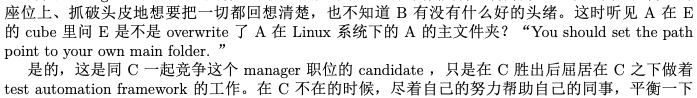
\includegraphics[width=.9\linewidth]{./pic/backups_plans_20210511_130349.png}
\end{center}

这里我们仍然可以一分为二地看待。就是一方面导师A作为这个组里的员工,确实有照顾我前导师mentor senior长老B的主观个人感受,而在那个旧新导师更替的关口,一定要批评我一下,这在先前当长老B与我的subversion的提交傻傻分不清楚的时候他也曾站出来平衡过。另一方面,我们仍然可以看作我的项目确实存在着怎样的问题。 

我们先来回顾一下,我亲爱的表哥眼中的少女心小弱弱成长的历史上、那几次经受振聋发溃的批评的历史案件!

\begin{center}

\includegraphics[width=.9\linewidth]{./pic/backups_plans_20210511_161158.png}
\end{center}

国内硕士研究生时导师在我开题告上对我的严厉批评,让我倍受痛楚,只想要做个冷血的学生,只求能够正常硕士毕业就好!

\begin{center}

\includegraphics[width=.9\linewidth]{./pic/backups_plans_20210512_100225.png}
\end{center}

\begin{center}

\includegraphics[width=.9\linewidth]{./pic/backups_plans_20210512_100246.png}
\end{center}

\begin{center}

\includegraphics[width=.9\linewidth]{./pic/backups_plans_20210512_100345.png}
\end{center}

\begin{center}

\includegraphics[width=.9\linewidth]{./pic/backups_plans_20210512_100319.png}
\end{center}

\begin{center}

\includegraphics[width=.9\linewidth]{./pic/backups_plans_20210512_100159.png}
\end{center}

11年2月当我回到家里向我亲爱的表哥表白,当我的舅舅故意将一顶顶罪恶的帽子向我头上砸来,当我的舅舅批评我的时候,我是全然不能接受哪怕是来自于自己深深信任的舅舅的严厉批评的!!!

\begin{center}
\includegraphics[width=.9\linewidth]{./pic/backups_plans_20210512_100728.png}
\end{center}

当那时我的舅舅对我的批评真正转化成自己可以意识到、可以落实到行动上的改变时,是又经历了一番自己的经历与领悟之后的事。 

\begin{center}
\includegraphics[width=.9\linewidth]{./pic/backups_plans_20210512_101244.png}
\end{center}

\begin{center}
\includegraphics[width=.9\linewidth]{./pic/backups_plans_20210512_101141.png}
\end{center}

12年5月,当我深爱的、我亲爱的表哥与播打了911之后,我恨过我表哥吗?当时的小弱弱是如何处理、过渡这段被自己亲爱的表哥播打911的事情呢?

\begin{center}
\includegraphics[width=.9\linewidth]{./pic/backups_plans_20210512_101333.png}
\end{center}

那时,被关在被自已称为“人间炼狱”的地方,只要我能够找出自己个性上存在的缺点,我就可以继续一如既往地相信我的亲爱的表哥!这就是我亲爱的表哥在我这里强大而又无卸可击、又给予着我深深爱恋的我亲爱的表哥在我这个当初的我亲爱表哥眼中的少女心小弱弱的强大存在!

\begin{center}
\includegraphics[width=.9\linewidth]{./pic/backups_plans_20210512_102518.png}
\end{center}

\begin{center}
\includegraphics[width=.9\linewidth]{./pic/backups_plans_20210512_102616.png}
\end{center}

而到后来,当我再长大一点儿、成熟一点、全然明白,我亲爱的表哥从来都是为我好、从来都是把选择权留给我、让我自己来作选择,便最终理解了我的舅舅和我亲爱的表哥最初的冷血、看似残忍做法。

我亲爱的表哥所曾给予我的这份爱,是这个世界上再也没有其它任何人可以给予我的,是我内心的深深索求与需要,所有今天的我选择回到我亲爱的表哥的身边,是再也没有任何其它外力可以阻止得了的。这是现在的最真实的感受。 

\begin{center}
\includegraphics[width=.9\linewidth]{./pic/backups_plans_20210512_100917.png}
\end{center}

那年刚过去的3月9日,当我写在《误会》里的澄清,也曾清楚地写到自己的接受别人批评困难的问题(“接受别人的批评很困难”)。 

那么导师A批评我的当时,我是如何反应的呢?

\begin{center}
\includegraphics[width=.9\linewidth]{./pic/backups_plans_20210512_103506.png}
\end{center}

原来那天下午四个小时左右的时间,我还曾被自己从新导师A的framework的源代码里抄过来的“@staticmethod”这个bug折腾过、浪费过时间哦?!

\begin{center}
\includegraphics[width=.9\linewidth]{./pic/backups_plans_20210512_103758.png}
\end{center}

导师A听见了我的神回复——他不曾知道我抄他的代码我抄了一行自己原本不需要的!所以他会笑着再问我可都弄懂了?

\begin{center}
\includegraphics[width=.9\linewidth]{./pic/backups_plans_20210512_104131.png}
\end{center}


\begin{center}
\includegraphics[width=.9\linewidth]{./pic/backups_plans_20210512_104021.png}
\end{center}

\begin{center}
\includegraphics[width=.9\linewidth]{./pic/backups_plans_20210512_104149.png}
\end{center}

这里我们再来回想一下,几个月前的春上、当我参考网站上代码写出密码设置为想要我亲近的表哥爱我一生一世(2514)的RTOS实时操控系统的作业,系里的大牛指出我们不应该抄网站上的代码的时候,我的态度是怎样的呢?

那么现在经历了这又一个抄别人的代码抄出来的bug之后,感受如何?!!!

这个对比与经历,可是看作是典型沉浸式长大、总是把别人的话当作过耳东风、必须经历过一些事情、有过一番相关联的经历之后,才能从经验、教训中吸取养份并成长的典型代表。

而这,也一再印证:对于我这样一个顽冥不化的沉浸式长大,我的舅舅、和我亲爱的表哥也是没有别的任何办法、除了用相对残忍的法律手段的!这里这些,就当是对自己个性的剖析吧。 

这里,这次,我就真的是全然接受了导师A的批评了吗?对于一个人个性中的长久存在,能够改变得这么快?我自己好像都还有些不信呢!

\begin{center}
\includegraphics[width=.9\linewidth]{./pic/backups_plans_20210512_104720.png}
\end{center}

这样看来,也才算正常吧。毕竟一个人的缺点没有那么容易轻易改变的。 

\begin{center}
\includegraphics[width=.9\linewidth]{./pic/backups_plans_20210512_105001.png}
\end{center}

\begin{center}
\includegraphics[width=.9\linewidth]{./pic/backups_plans_20210512_105033.png}
\end{center}

\begin{center}
\includegraphics[width=.9\linewidth]{./pic/backups_plans_20210512_105046.png}
\end{center}

而导师A那时还特意留在公司,应该也是因为几个月前的3月我已经特意强调过自己个性中的这个缺点吧,公司里制造爆点、打舆论,又如何会放过这个细节?

\begin{center}
\includegraphics[width=.9\linewidth]{./pic/backups_plans_20210512_105449.png}
\end{center}

可是,作为实习生的我要求导师A这么做了吗,从一开始、就是正式员工A全然领悟公司在这个特殊时期招他入公司的深意呀、他职场老油条、在尖人等警犬的一再点示下深得三星公司暑假炒作深意,他当然是为得到他在三星公司职场的发展全然配合公司需求,来全力加入并点爆、来制造燃点爆点来炒作舆论的呀! 

我们接下来看看三星公司里、site里警犬的攻效如何、警犬的鼻子灵不灵呢?

\begin{center}
\includegraphics[width=.9\linewidth]{./pic/backups_plans_20210512_105614.png}
\end{center}

这是新专业里的实习生、知识体悟里的感受。

\begin{center}
\includegraphics[width=.9\linewidth]{./pic/backups_plans_20210512_111724.png}
\end{center}

\begin{center}
\includegraphics[width=.9\linewidth]{./pic/backups_plans_20210512_111818.png}
\end{center}

\begin{center}
\includegraphics[width=.9\linewidth]{./pic/backups_plans_20210512_113149.png}
\end{center}

这里我们也来对比与先前导师mentor senior长老B的实习感受。 

那年夏天、自己在三星公司里的实习,公司里为自己按排的前导师mentor senior长老B究竟算是什么样的存在呢?

\begin{center}
\includegraphics[width=.9\linewidth]{./pic/backups_plans_20210512_112101.png}
\end{center}

\begin{center}
\includegraphics[width=.9\linewidth]{./pic/backups_plans_20210512_112040.png}
\end{center}

呵呵,这里,我们也再来体会一次一两个周之前公司里曾经所挖过的天坑bug.

对于警犬——尖人的忽然前来打招呼、查岗与询问、更重要的传达公司里欲要炒作燃点爆点的需求,我显然是反应不过来的,我的反应是什么呢?

可以看出,当年的我在感受人情世故方面仍然存在着一定程度上的错位。

\begin{center}
\includegraphics[width=.9\linewidth]{./pic/backups_plans_20210512_111026.png}
\end{center}

\begin{center}
\includegraphics[width=.9\linewidth]{./pic/backups_plans_20210512_111048.png}
\end{center}

不记得是什么时候了,可能先前跟着导师长老B、关系还不太缰的时候吧,她早上来找我去喝咖啡,被我拒绝了,我不需要、至少是早上不需要的。 

\begin{center}
\includegraphics[width=.9\linewidth]{./pic/backups_plans_20210512_111123.png}
\end{center}

\begin{center}
\includegraphics[width=.9\linewidth]{./pic/backups_plans_20210512_112652.png}
\end{center}

这里有一种强烈的回忆起来的感受,就是那个夏天、就像那上班第一天、两个女人通过她们自己的战争、把一个实习生架空在大家都能够注意得到、看得见的位置上,这个公司、这个site感受把我盯得极紧,我就完全沦为那个夏天实习的风暴、舆论焦点。

那么、对于昨天、前一天下班前帮我review交叉项目、review时曾刻意批评过我的自己的新导师A呢?

\begin{center}
\includegraphics[width=.9\linewidth]{./pic/backups_plans_20210512_114515.png}
\end{center}

周四中午(新导师A将约十天前布置的项目拖到了新一周的周三傍晚才review),导师A在不在公司里吃饭。

\begin{center}
\includegraphics[width=.9\linewidth]{./pic/backups_plans_20210512_113036.png}
\end{center}

正常情况下周二到周四的中午三餐饭公司里是管饭吃的,而人们愿意不愿意、有没有脸面在公司里吃饭,也全看公司里的氛围、看眼色行事。 

那天晚上我被新导师A批评了,我自己不愿意在公司里吃饭,跑出去吃东西透气了,那也是我自己的自愿。但是后来公司里的警犬、风向标——尖人已经不允许我再在公司里吃晚饭了,这是后话。 

那么可以清楚地看到,当以尖人为代表的人想要导师A发动炒作与我的绯闻舆论的时候,前一天晚上导师A也曾特意再等到我回公司才离开,但我与他并没有任何更多的联接。

所以第二天上午、当导师A去问对面实习生E一个什么想法的时候,我不再去听他们的谈话,而是自顾自地打电话询问先前某次看病账单的事了。 

\section{我最亲爱的表哥(4)}
\label{sec:orge5c662d}

《这个是:最终结局——爱情婚姻的归属摆在这里,等这所有的内容全部写完,我会回来把这部分写得更好点儿!》

亲爱的表哥,写到这里,我终于是完成了我们共同完成的一件壮举:破除三大中文网站逼良为娼的产业化操作,将他们如此炒作自家网红、并最终逼良为娼的黑色产业链彻底白菜化,让他们这一见不得光的暗箱操作彻底见光死、让他们的这个产业链在广大小市民、在老百姓心目中遍地开花、了然于胸、一见便知、心知肚明,让越来越少的女性、女留学生们陷入到我曾经所遭遇的这些困境中来!

亲爱的表哥,这件事情、在你(和舅舅)的发动、在我快速成长与无限配合下,我们终于是合作完成了一件壮举,我们做到了:为往事干杯,为我们自己干一杯!

到2021年这个春天,我终于明白,09年秋季学期、舅舅不早不晚在我统计专业的最后一个学期、为我从韩国搬回来的亲爱的表哥你,就是真真正正要表哥你来作我的坚强后盾来着!不是早年间12年表哥你亲手播打911后我在人间炼狱里自己反省出来的自已是寄生草寄生虫,舅舅帮我搬回来的就是真真正正、我内心里最想要的,我的矿世爱情和我今生的终身归属!

有一种感动——惊心动魄,有一种遭遇——万劫不复,当我们遭遇了爱情、追寻过梦想、历经了沧伤,当我们重新回到梦开始的地方、回到我们分开出发的起点,亲爱的表哥,你还在等我吗,你还可以接纳今天的我吗?

亲爱的表哥,你可以接纳现在的我吗?你是否也如我般曾经沧海?你的沧海里是否可以容下我的眼泪?

亲爱的表哥,我们——你和我,有一个十年之约,我会欣然前往赴约,你准备好了吗?

这一次,这个月底(还有几天到这个月的31号,我就出发开车返回亲爱的表哥你所在的Pullman的土地上),我要回到亲爱的表哥你所在的Pullman的土地上,申请回到亲爱的表哥你所在的WSU的校园里读博士研究生,我要作亲爱的表哥你房间里的女主人,我想要陪你一起、我们共同走完余生!

亲爱的表哥,这次,我再也不会再走丢,你也一定要等着我,等我回到你身边,不许再播打什么911,不许你逃跑\textasciitilde{}!!!

昨天是你毕业四周年的日子,恭喜你,恭喜我们 \textasciitilde{}! 

毕业四年了,工作几年了。 

\textbf{亲爱的表哥,你准备好,准备好今年可以娶我了吗?!!!我等着!!!}

\section{成长的故事 -- 我和表哥}
\label{sec:org7f2af0f}
\begin{itemize}
\item 2011年11月4日,当三大中文媒体对我的人肉已经伤及我自身生活,我必须站出来澄清自己, in Part 1, (San Jose, CA);

\begin{center}
\includegraphics[width=.9\linewidth]{./pic/dreamer1.png}
\end{center}
\item 4/19/2012 - 6/17/2012, in Part 1, 第二次写至统计专业OPT实习结束(San Jose, CA);

\begin{center}
\includegraphics[width=.9\linewidth]{./pic/dreamer2.png}
\end{center}
\item 2014年夏天,写于SJSU Library (San Jose State University Public Library, San Jose, CA)

\begin{center}
\includegraphics[width=.9\linewidth]{./pic/dreamer30.png}
\end{center}
\item 2/13/2015 - 12/17/2015(?, Moscow, ID; either and or not San Jose State University Public Library, San Jose, CA)

\begin{center}
\includegraphics[width=.9\linewidth]{./pic/dreamer3.png}
\end{center}

\item I will reorganize the four pdfs, and emphasize keys issues and situations of the whole process, while at the same time to help major population understand what's going on, and what's inside opinions. 虽然这个成长的故事系列是以2011年当三大中文网站(mitbbs.com, wenxuecity.com and backchina.com)中文媒体对我的人肉与网上评论伤及我的正常生活时,我站出来开始写自己的自传,并分四次在四个不同的时间段,不同舆论或事件压力下或是网上澄清,或是网上求助以便能帮我泄掉一部分当时自己的压力,分四次于不同的地点纪录了的自己的主要生活,纪录到2015年计算机硕士学位结束。
\item 这一次,这里,我会以事件主要人物及其相关主要事迹的人物列传、或/和大事记、大冲突记的形式来重新组织语言,重述我的整个成长史与大事记、大冲突记,来帮助自己成长、并帮助社会大众认清事情所有环节真相的目的。但鉴于时间有限,我会以剧情梗概的形式每天大致纪录与一个相关人物某件或某几件事的进展、或一天一两个主要事件,并将已经完成了的四个部分作为原始事件纪录的细节参考供索引,并争取做到每日更新一篇,到我把先前与这个教授舅舅的所有冲突的这件事情具体讲述清楚,以供大家共同去探讨事情的真相到底如何,有一个更能为大家所接受或理解的底层社会小人物的心灵成长史。
\end{itemize}
\end{document}